% Single Image 
\begin{figure}
	\centering
	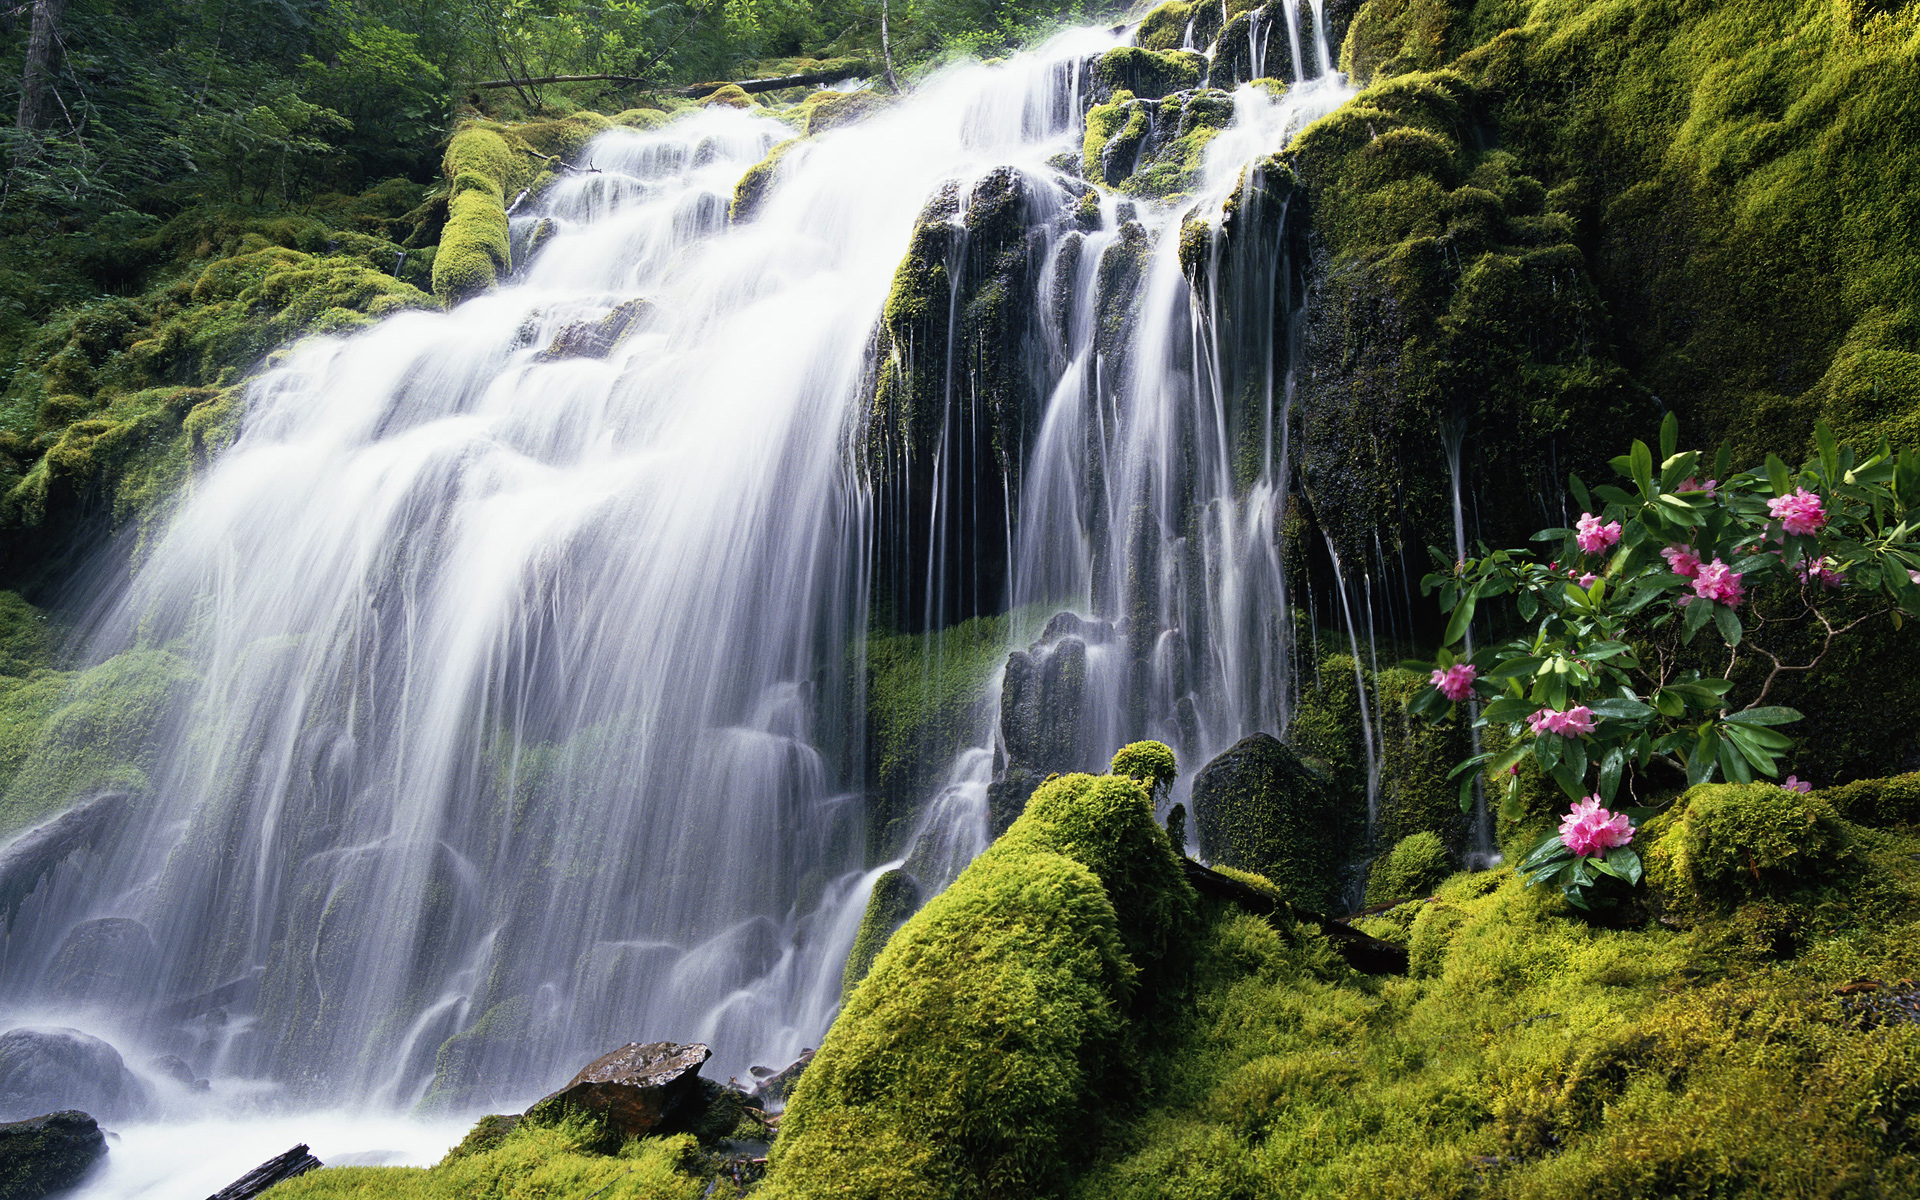
\includegraphics[width=0.7\linewidth]{image2}
	\caption{Caption of fig. 1.}
	\label{fig:image2}
\end{figure} 

% Multiple Images 
\begin{figure}
\centering
\begin{subfigure}[b]{0.45\textwidth}
  \centering
  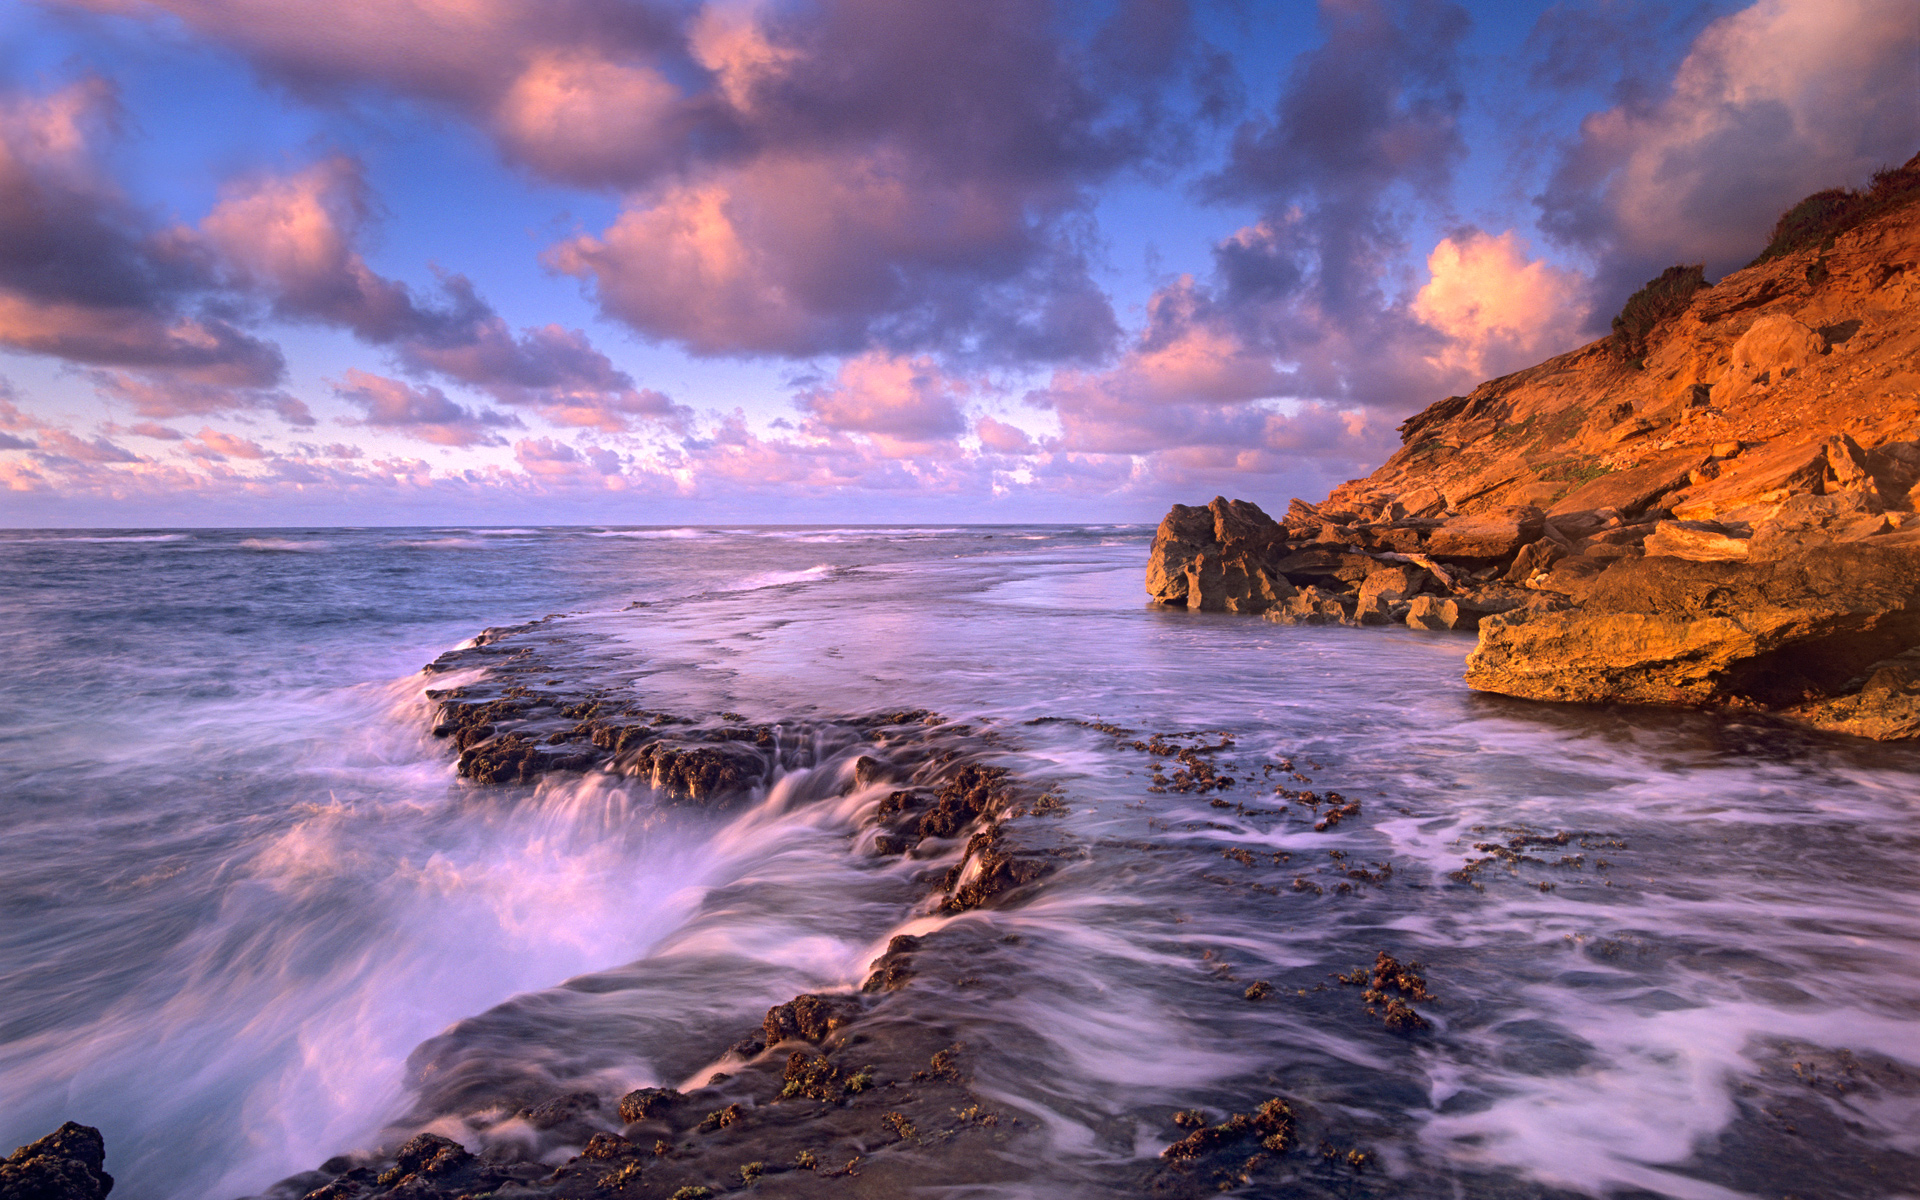
\includegraphics[width=\textwidth]{image1}
  \caption{}
  \label{fig:im1}
 \end{subfigure}
~
\begin{subfigure}[b]{0.45\textwidth}
  \centering
  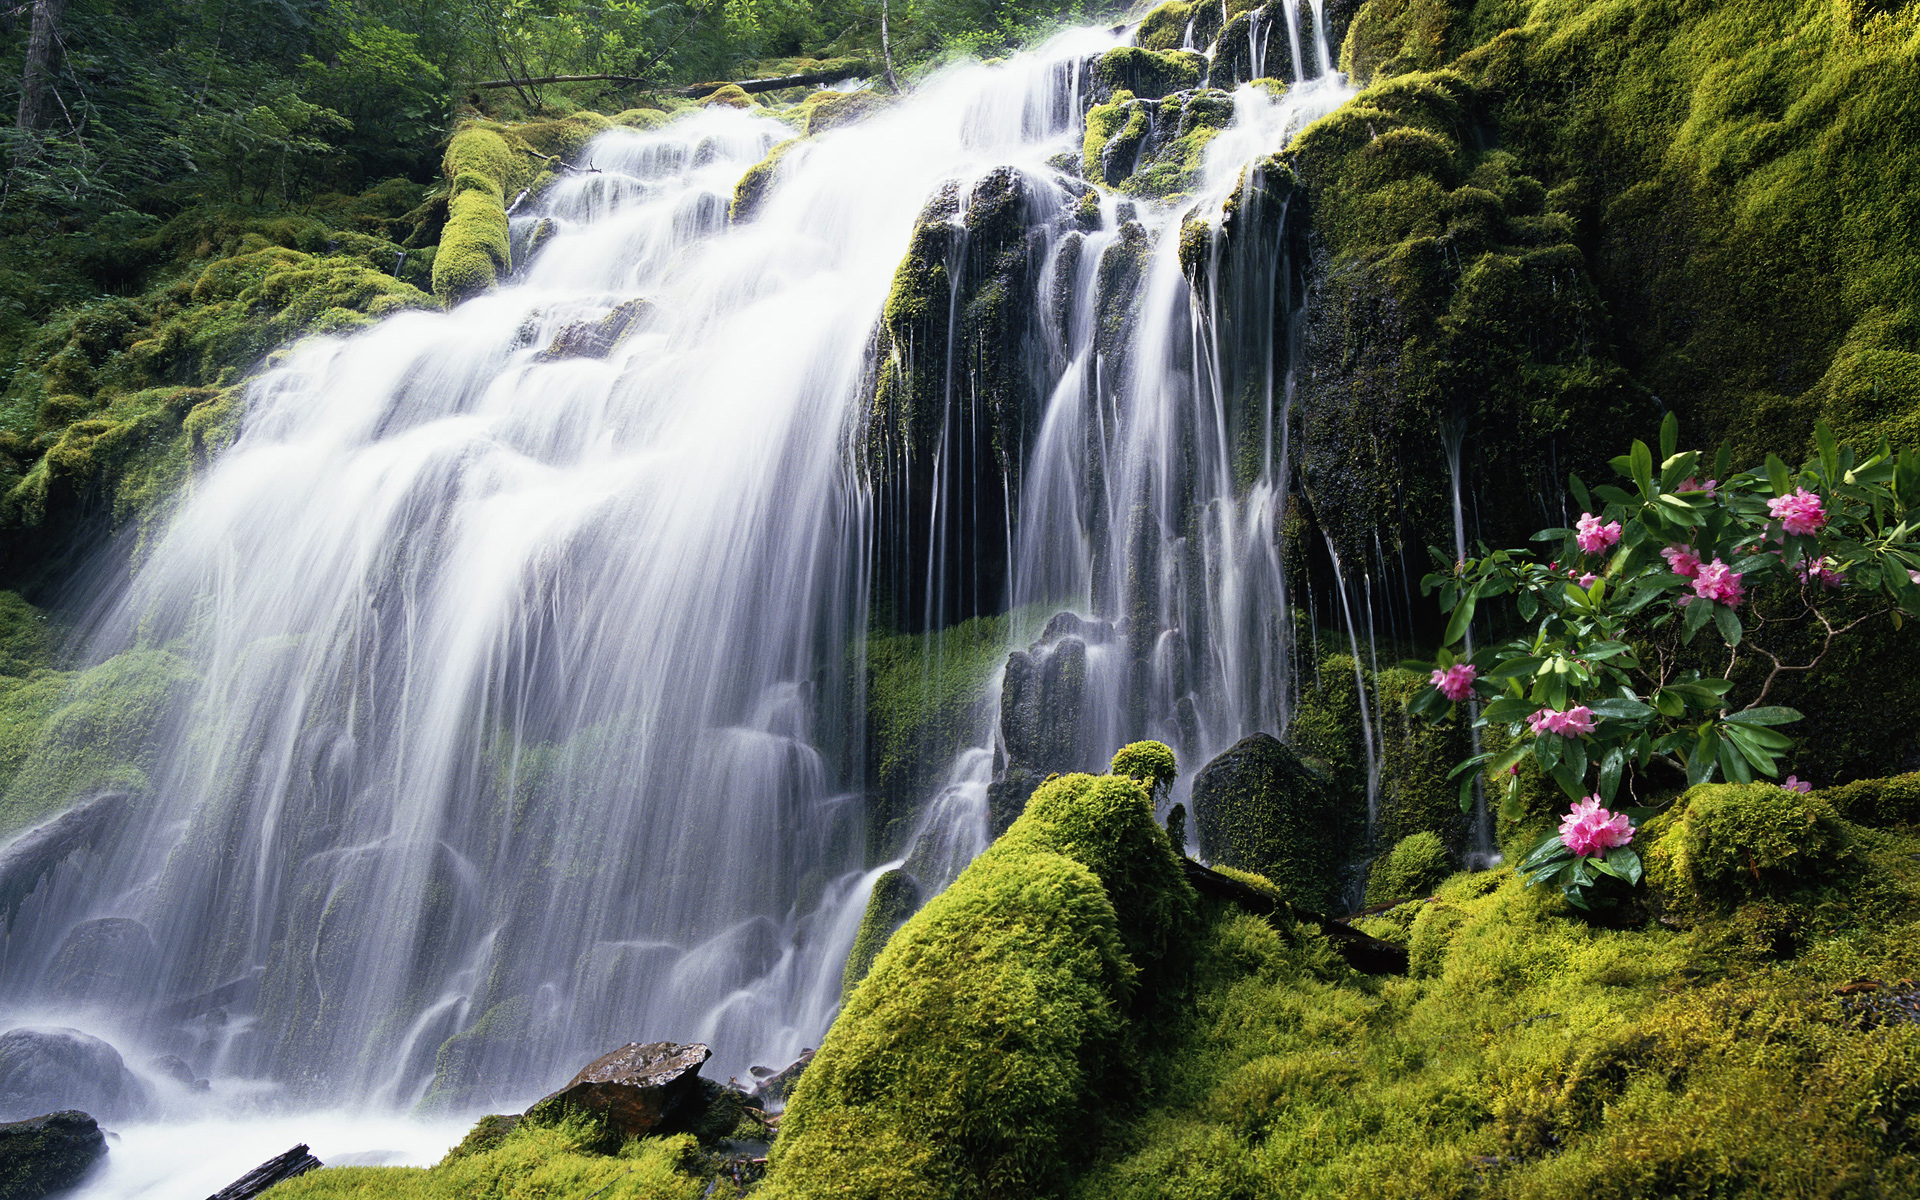
\includegraphics[width=\textwidth]{image2}
  \caption{}
  \label{fig:im2}
\end{subfigure}
\caption{Two figure side by side}
\label{fig:subfigs cap}
\end{figure}
